\documentclass[../main/main.tex]{subfiles}

\begin{document}

\section{Sphinx}

\subsection{Setup}

Using Sphinx requires only one simple Python package, \lstinline|sphinx|,
however, there also are other additional packages such as the
\lstinline|sphinx_rtd_theme| that we will install. 

\subsection{Quickstart}

We will use \lstinline|sphinx-quickstart| to quickly setup a Sphinx project
thereby gaining build files like a Makefile. For this project we need a vital
extension called \lstinline|autodoc|, thus we need enter \lstinline|y|, if we
are asked, whether we want to include it. 

The command should be entered in the root directory of the project, therefore
we will also enter \lstinline|docs| as the root path for the documentation, as
we do not want to mess up the source files with the documentation files. 

An example is shown below in Listing \ref{lst:sphinx-quickstart}

\begin{lstlisting}[caption=Example Sphinx-Quickstart, label=lst:sphinx-quickstart]
>>> sphinx-quickstart
Welcome to the Sphinx 1.3.1 quickstart utility.

Please enter values for the following settings (just press Enter to
accept a default value, if one is given in brackets).

Enter the root path for documentation.
> Root path for the documentation [.]: docs

You have two options for placing the build directory for Sphinx output.
Either, you use a directory "_build" within the root path, or you separate
"source" and "build" directories within the root path.
> Separate source and build directories (y/n) [n]:

Inside the root directory, two more directories will be created; "_templates"
for custom HTML templates and "_static" for custom stylesheets and other static
  files. You can enter another prefix (such as ".") to replace the underscore.
  > Name prefix for templates and static dir [_]:

  The project name will occur in several places in the built documentation.
  > Project name: Trackit
  > Author name(s): Gary Ye

  Sphinx has the notion of a "version" and a "release" for the
  software. Each version can have multiple releases. For example, for
  Python the version is something like 2.5 or 3.0, while the release is
  something like 2.5.1 or 3.0a1.  If you don't need this dual structure,
  just set both to the same value.
  > Project version: 0.1
  > Project release [0.1]: 1.0

  If the documents are to be written in a language other than English,
  you can select a language here by its language code. Sphinx will then
  translate text that it generates into that language.

  For a list of supported codes, see
  http://sphinx-doc.org/config.html#confval-language.
  > Project language [en]:

  The file name suffix for source files. Commonly, this is either ".txt"
  or ".rst".  Only files with this suffix are considered documents.
  > Source file suffix [.rst]:

  One document is special in that it is considered the top node of the
  "contents tree", that is, it is the root of the hierarchical structure
  of the documents. Normally, this is "index", but if your "index"
  document is a custom template, you can also set this to another filename.
  > Name of your master document (without suffix) [index]:

  Sphinx can also add configuration for epub output:
  > Do you want to use the epub builder (y/n) [n]:

  Please indicate if you want to use one of the following Sphinx extensions:
  > autodoc: automatically insert docstrings from modules (y/n) [n]: y
  > doctest: automatically test code snippets in doctest blocks (y/n) [n]:
  > intersphinx: link between Sphinx documentation of different projects (y/n) [n]:
  > todo: write "todo" entries that can be shown or hidden on build (y/n) [n]:
  > coverage: checks for documentation coverage (y/n) [n]:
  > pngmath: include math, rendered as PNG images (y/n) [n]:
  > mathjax: include math, rendered in the browser by MathJax (y/n) [n]:
  > ifconfig: conditional inclusion of content based on config values (y/n) [n]:
  > viewcode: include links to the source code of documented Python objects (y/n) [n]:

  A Makefile and a Windows command file can be generated for you so that you
  only have to run e.g. `make html' instead of invoking sphinx-build
  directly.
  > Create Makefile? (y/n) [y]:
  > Create Windows command file? (y/n) [y]:

  Creating file docs/conf.py.
  Creating file docs/index.rst.
  Creating file docs/Makefile.
  Creating file docs/make.bat.

  Finished: An initial directory structure has been created.

  You should now populate your master file docs/index.rst and create other documentation
  source files. Use the Makefile to build the docs, like so:
     make builder
     where "builder" is one of the supported builders, e.g. html, latex or linkcheck.
\end{lstlisting}%$

\subsection{Generating the Documentation}

Sphinx works with \lstinline|*.rst| files, which can be seen as a script files,
in which we use a certain syntax to produce a certain documentation. 

However we can also use inline code documentation so that we don't have to
separate our source files from our documentation files by using the
\lstinline|autodoc| package. We merely have to write which kind of modules,
class, ..., have to be included in our documentation. As this can be a tedious
process to list them all, Sphinx has also included a helper script
\lstinline|sphinx-apidoc|, which we will use to generate the corresponding
\lstinline|rst| files. 

\begin{lstlisting}
>>> sphinx-apidoc -o docs app
Creating file docs/app.rst.
Creating file docs/app.crawling.rst.
Creating file docs/app.forms.rst.
Creating file docs/app.models.rst.
Creating file docs/app.models.facebook.rst.
Creating file docs/app.models.twitter.rst.
Creating file docs/app.views.rst.
Creating file docs/modules.rst.
\end{lstlisting}

To use \lstinline|autodoc| properly, it also needs to include the packages, thus
we need to set the \lstinline|PYTHONPATH| appropriately. In the
\lstinline|docs/conf.py|, we must also include the root directory of the project
into the \lstinline|PYTHONPATH|. 

\begin{lstlisting}[caption=docs/conf.py, label=lst:sphinxconfpy]
sys.path.insert(0, os.path.abspath('../'))
\end{lstlisting}

Basically, we can just enter the \lstinline|docs| directory now, and enter the
following \lstinline|make| command, in order to generate all files. 

\begin{lstlisting}
make html
\end{lstlisting}

\subsection{\lstinline|index.rst|}

For creating an aesthetic documentation tree, just use the following lines in
the \lstinline|index.rst| file: 

\begin{lstlisting}
.. toctree::
  :maxdepth: 2

  app
\end{lstlisting}

Where \lstinline|app| is the root module. A tree of \lstinline|maxdepth| = 2,
will be created recursively.  


\subsection{Read The Docs (optional)}
An extraordinary theme that guranteely gets you bonus points:

\begin{lstlisting}
pip install sphinx_rtd_theme
\end{lstlisting}

Find the line with \lstinline|html_theme|, and replace it with the following
three lines, provided in \ref{lst:sphinx_rtd}

\begin{lstlisting}[caption=docs/conf.py,label=lst:sphinx_rtd]
import sphinx_rtd_theme
html_theme = "sphinx_rtd_theme"
html_theme_path = [sphinx_rtd_theme.get_html_theme_path()]
\end{lstlisting}

The default theme should be \lstinline|alabaster|, however, a picture of the
Readthedocs theme should convince everyone. 

\begin{figure}
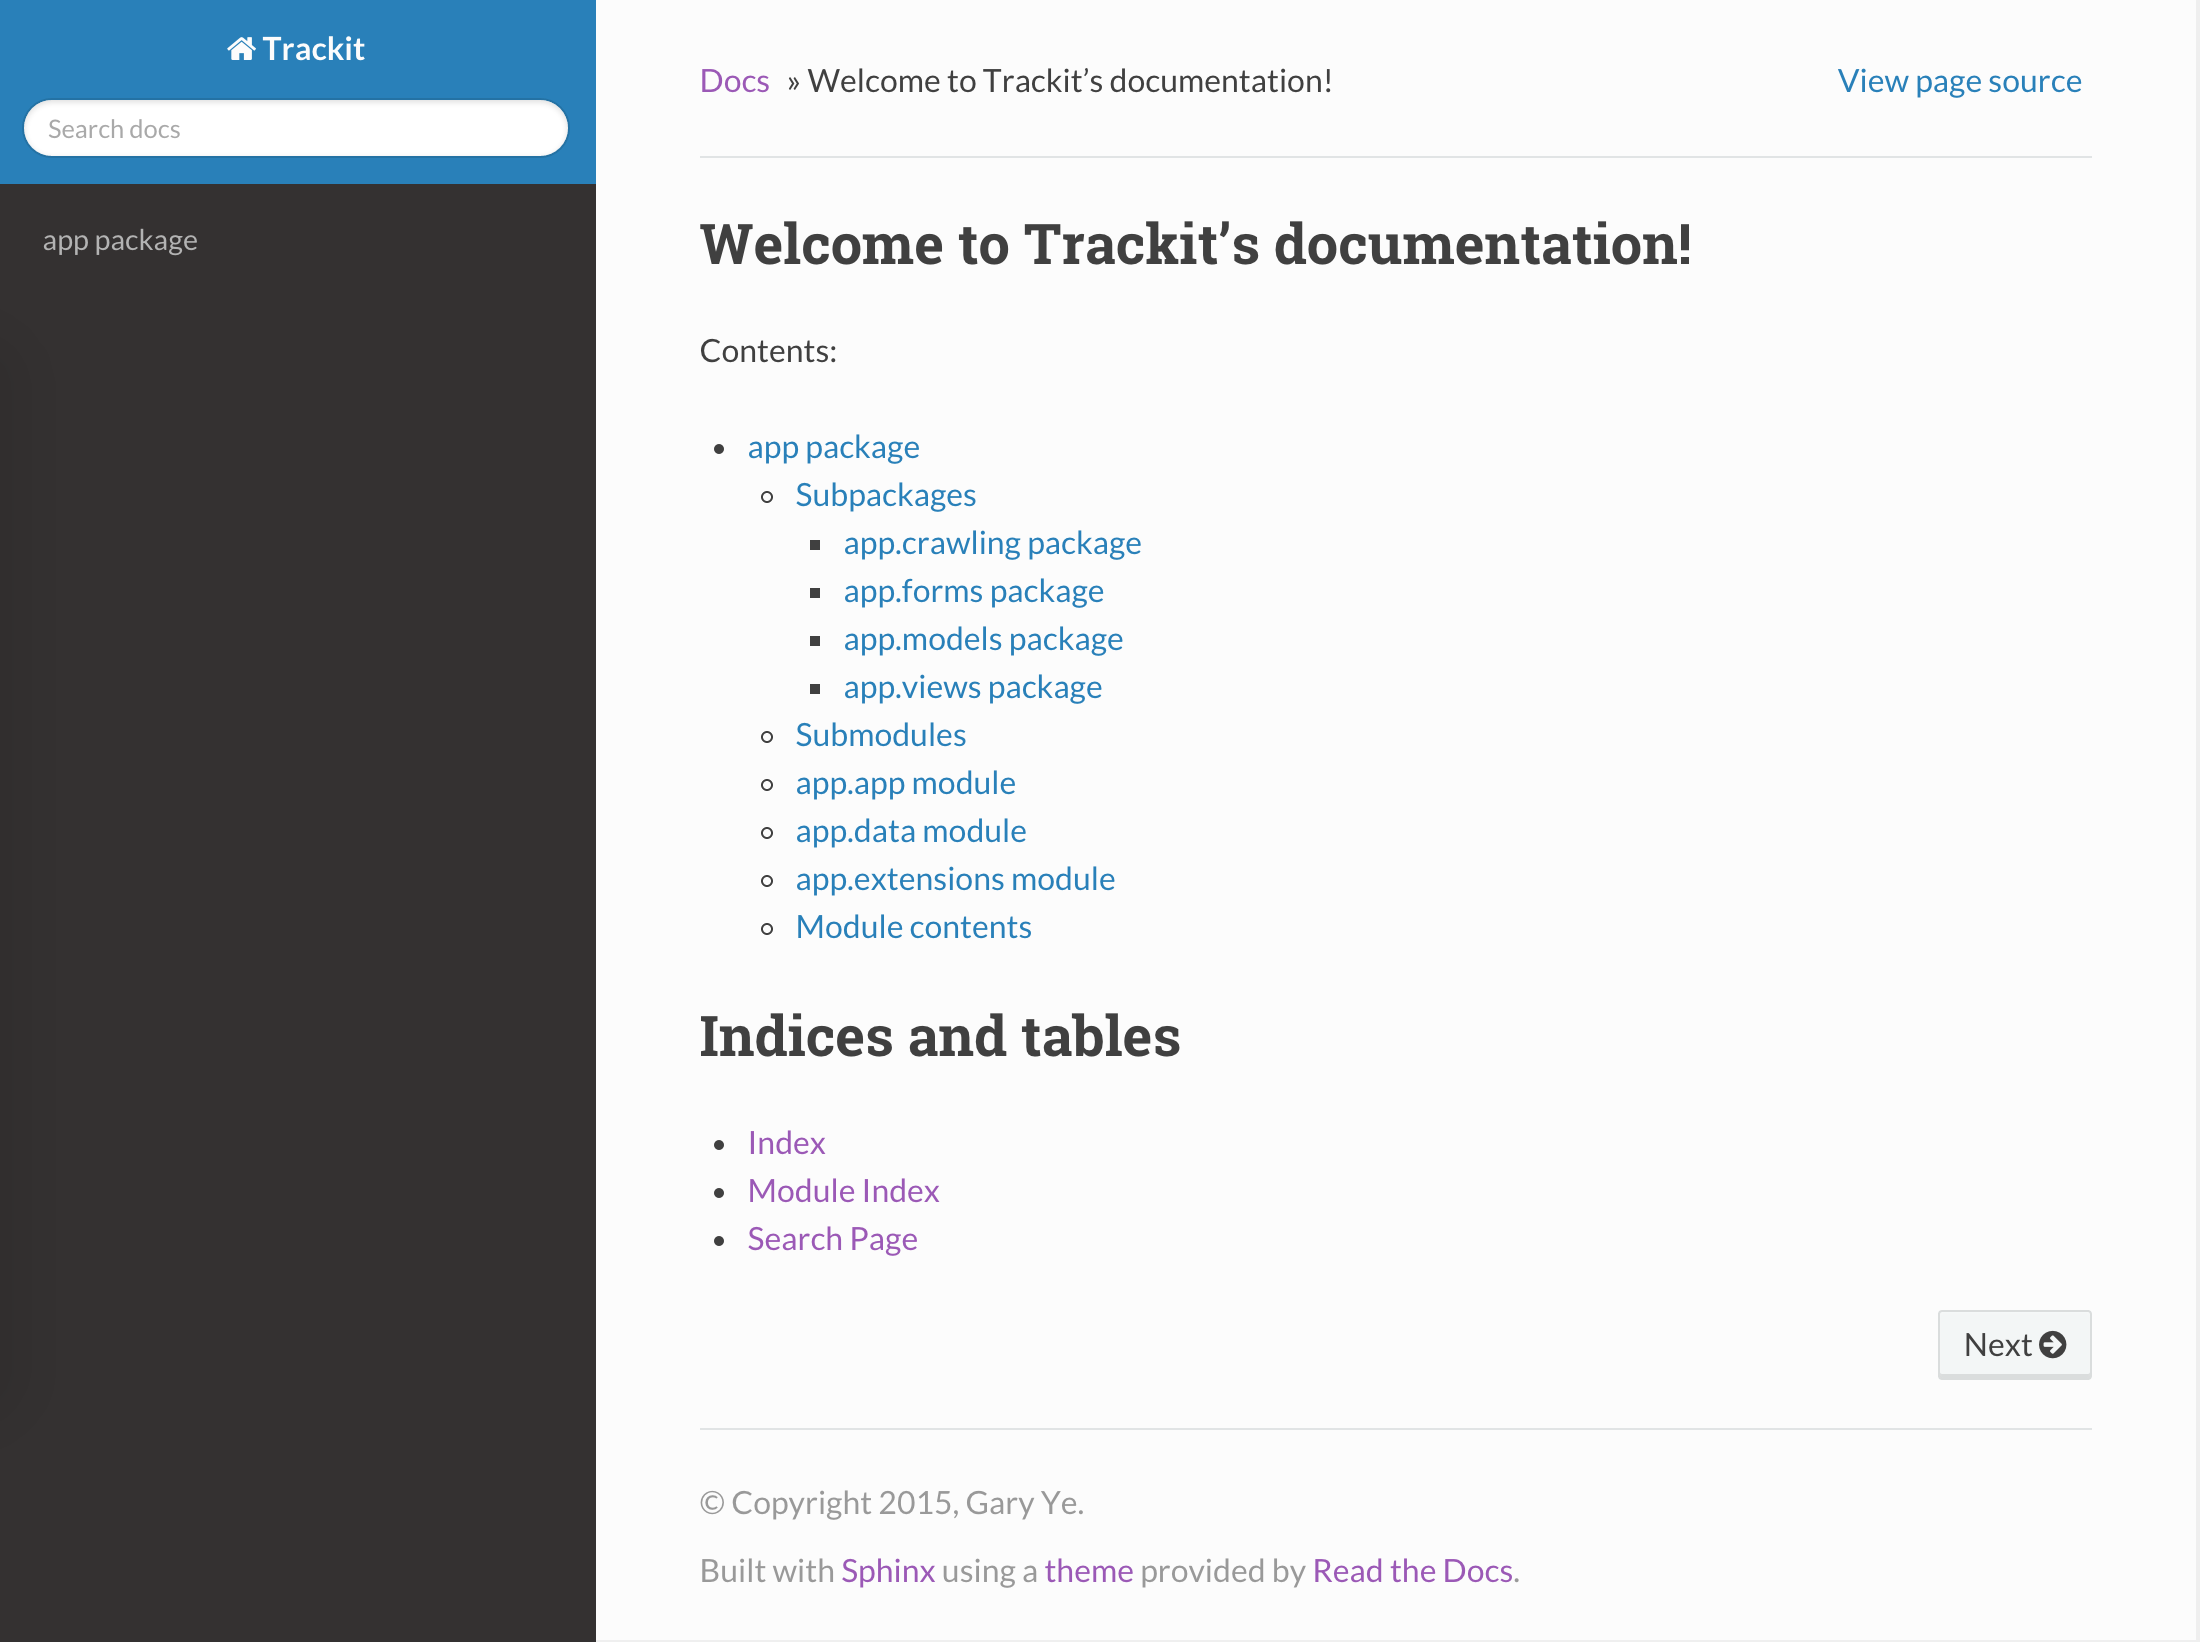
\includegraphics[]{../figures/rtd_sphinx.png}
\end{figure}

\subsection{Documentation Syntax}

The official way to document the code is provided in \cite{sphinx:rest}.

\end{document}
